%--------------------------------------------------
% \documentclass[runningheads,a4paper]{llncs}
%-------------------------------------------------- 
\documentclass[a4paper]{llncs}
\usepackage{amssymb}
\setcounter{tocdepth}{3}
\usepackage{graphicx}

\usepackage{url}
%--------------------------------------------------
% \urldef{\mailsa}\path||
% \urldef{\mailsb}\path||
% \urldef{\mailsc}\path||
%-------------------------------------------------- 
\urldef{\mailsa}\path|cobain@turing.csie.ntu.edu.tw|
\urldef{\mailsb}\path|cmtsai@mail.lis.ntu.edu.tw|
\urldef{\mailsc}\path|jhsiang@ntu.edu.tw|
\newcommand{\keywords}[1]{\par\addvspace\baselineskip
\noindent\keywordname\enspace\ignorespaces#1}

%--------------------------------------------------
% % Traditional-Chinese support
%-------------------------------------------------- 
%--------------------------------------------------
% \usepackage[cjkbg5]{ucs}
% \usepackage[utf8x]{inputenc}
% \usepackage[C00,T1]{fontenc}
% \DeclareFontSubstitution{C00}{bsmi}{m}{n}
% \newcommand\zhtw[1]{\bgroup\fontencoding{C00}\fontfamily{ming}\selectfont%
% \SetUnicodeOption{cjkbg5}#1\egroup}
%-------------------------------------------------- 
\newcommand\zhtw[1]{}

\usepackage{amsmath}
\usepackage{pst-all} % PSTricks
\usepackage{com.braju.graphicalmodels} % The package that really does the hard work
\catcode`\@=11%

\usepackage{color}
\newcommand{\comment}[1]{{\color{red}#1}}

\begin{document}
\mainmatter  % start of an individual contribution
\title{Relevance Model Revisited: With Multiple Document Representations}
\titlerunning{Relevance Model Revisited: With Multiple Document Representations}

\author{Ruey-Cheng Chen\and Chiung-Min Tsai\and Jieh Hsiang}
%--------------------------------------------------
% \author{XXXXXXXX\and XXXXXXXX\and XXXXXXXXX}
%-------------------------------------------------- 
\authorrunning{Relevance Model Revisited: With Multiple Document Representations}

% the affiliations are given next; don't give your e-mail address
% unless you accept that it will be published
\institute{National Taiwan University,\\
1 Roosevelt Rd. Sec. 4, Taipei 106, Taiwan\\
\mailsa\\
\mailsb\\
\mailsc\\
}

%--------------------------------------------------
% \institute{XXXXXXXX\\
% XXXXXXXX\\
% \mailsa\\
% \mailsb\\
% \mailsc\\
% }
%-------------------------------------------------- 

%
% NB: a more complex sample for affiliations and the mapping to the
% corresponding authors can be found in the file "llncs.dem"
% (search for the string "\mainmatter" where a contribution starts).
% "llncs.dem" accompanies the document class "llncs.cls".
%

\toctitle{}
\tocauthor{}
\maketitle
\documentclass{article}[12pt]
%--------------------------------------------------
% \documentclass{sig-alternate}
%-------------------------------------------------- 
\usepackage{algorithm}
\usepackage{algorithmic}
\usepackage{graphicx}
%--------------------------------------------------
% \documentclass{acm_proc_article-sp}
%-------------------------------------------------- 
\newcommand\url[1]{\texttt{#1}}

\def\sharedaffiliation{%
\end{tabular}
\begin{tabular}{c}}

\begin{document}
\title{Proposal for NSC Graduate Student Study Abroad Program}
%--------------------------------------------------
% \subtitle{Working Draft}
%-------------------------------------------------- 
\author{Ruey-Cheng Chen\\Dept. of Computer Science and Information Engineering\\National Taiwan University, Taiwan}
%--------------------------------------------------
% \numberofauthors{1} %  in this sample file, there are a *total*
% % of EIGHT authors. SIX appear on the 'first-page' (for formatting
% % reasons) and the remaining two appear in the \additionalauthors section.
% %
% \author{
% \alignauthor Ruey-Cheng Chen\\
%   \email{cobain@turing.csie.ntu.edu.tw}\\
%   \affaddr{Dept. of Computer Science and Information Engineering}\\
%   \affaddr{National Taiwan University, Taiwan}
% }
%-------------------------------------------------- 
%--------------------------------------------------
% \date{30 July 1999}
%-------------------------------------------------- 
\maketitle

\section{Biography}

Ruey-Cheng Chen\footnote{\url{http://wkd.iis.sinica.edu.tw/$\sim$cobain}}, who
received his B.S. and M.S. degrees in Department of Computer Science and
Information Engineering, National Taiwan University, has been working for
Institute of Information Science, Academia Sinica since 2004.  Currently,
Ruey-Cheng works as a research assistant in the Web Knowledge Discovery Lab
lead by Dr. Lee-Feng
Chien\footnote{\url{http://www.iis.sinica.edu.tw/$\sim$lfchien/}}, and also as
a graduate student of Prof. Jieh
Hsiang\footnote{\url{http://www.csie.ntu.edu.tw/$\sim$hsiang/}}.  His research
interests include text mining, cross-language information retrieval, and
machine translation.

Over the past five years, Ruey-Cheng has actively joined two research projects
sponsored by NSC, \emph{LiveTrans} and \emph{LiveImage}, where he is
responsible for most of the experimentation and system implementation jobs.
Achievements of the projects involve scientific reports and live systems open
to public access.  The details of these projects are presented in the following
sections.

\subsection{LiveTrans}

The LiveTrans\footnote{\url{http://wkd.iis.sinica.edu.tw/LiveTrans/}} system is
a meta-search engine that offers cross-language search capability for retrieval
of both Web pages and images.  One of the major bottlenecks in cross-language
information retrieval applications is the lack of appropriate and up-to-date
bilingual dictionaries, which contain the translations of popular query terms,
such as new terminology and proper names. In order to discover more effective
query translations, the LiveTrans system was developed to demonstrate a
state-of-the-art technology for automatically translating search terms not
included in the bilingual dictionaries with an innovative Web mining technique.
A few technical papers regarding the research have been published on premier
conference proceedings, such as SIGIR'04, ACL'04 and JCDL'04, and journals,
such as ACM TOIS'04 and ACM TALIP'02, which have shown the system's great
potential to benefit the development of cross-language information retrieval
research.

\paragraph{Publication}
\begin{itemize}
  \item Pu-Jen Cheng, Jei-Wen Teng, Ruei-Cheng Chen, Jenq-Haur
  Wang, Wen-Hsiang Lu, Lee-Feng Chien, ``Translating Unknown Queries with Web
  Corpora for Cross-Language Information Retrieval,'' SIGIR 2004: 146-153.
\end{itemize}

\subsection{LiveImage}

The increasing demand for high-performance Web image search engines is being
driven by the rapid growth in the number of Web users and in the availability
of image collections on the Web. It's very easy to retrieve a very large number
of images by submitting a short query to a Web search engine. Unfortunately,
the returned images are not well organized in a conceptually meaningful way. To
help users find images in a conceptually simple way, we propose an approach for
organizing retrieved images based on auto-generated relevant concepts. The
images listed in the retrieved results are organized according to their
similarity to the relevant concepts, which makes it easier for users to locate
images of interest with the corresponding concept names and relevant images.

Our goal is to discover meaningful concepts relevant to Web image queries.
Collecting and organizing such relevant concepts manually is infeasible due to
the dynamic nature of the Web environment. We are interested in developing an
automatic approach that organizes users' query terms into auto-generated
subject categories. As users' queries are short and new queries appear all the
time, our problem is to assign effective concept categories to users' queries
and improve their search performance, even if the given queries have never
appeared before. The proposed approach is a well-integrated set of innovative
techniques, including relevant concept finding, query clustering, and query
classification. A meta search engine,
LiveImage\footnote{\url{http://wkd.iis.sinica.edu.tw/LiveImage/}}, based on the
proposed approach is implemented and tested through extensive experiments. The
experiment results show that the performance of Web image retrieval can be
effectively improved with the proposed approach.

\paragraph{Publication}
\begin{itemize}
  \item Ruey-Cheng Chen and Pu-Jen Cheng, ``Discovering Relevant Concepts for
  Web Image Search,'' In the International Computer Symposium 2006, Taipei,
  Taiwan.  \item Shuo-peng Liao, Pu-Jen Cheng, Ruey-Cheng Chen and Lee-Feng
  Chien, ``LiveImage: Organizing Web Images by Relevant Concepts,'' In the
  Workshop on the Science of the Artificial 2005, pp. 210-220, Hualien, Taiwan,
  December 2005.  
\end{itemize}

\subsection{Awards}

During the fall of 2007, Ruey-Cheng Chen worked as a teaching assistant of
Prof. Pu-Jen Cheng\footnote{\url{http://www.csie.ntu.edu.tw/$\sim$pjcheng}} in
one of his course ``Web Retrieval and
Mining''\footnote{\url{http://irlab.csie.ntu.edu.tw/wm2007/}}.  Ruey-Cheng
later received the Excellent Teaching Assistant Award in early summer of
2008, from Department of Computer Science and Information Engineering, National
Taiwan University.
  
\section{The ICT Story Representation and Management Project}

\subsection{Overview}

The Story Representation and Management projects
\footnote{\url{http://ict.usc.edu/projects/story\_representation\_and\_management/C42}}
at ICT are aimed at developing technologies and methodologies for supporting
the rapid development of U.S.  Army training applications involving the
collection, analysis, and use of first-person narratives of real-world
experiences (stories). Research on this project focuses on the following
problems: 

\begin{itemize} \item 
Automated story capture -- Technologies for
automatically recognizing when people are telling stories about their
experiences in written text (e.g., Internet weblogs) using statistical natural
language processing. \item Story retrieval interfaces -- Technologies for
identifying stories from the Internet and other large text repositories that
directly address specific training objectives, using semantic and syntactic
text processing techniques.  \item Story interpretation -- Techniques for
integrating automated commonsense inference into the processing of narrative
text documents, and methodologies for creating very large scale commonsense
knowledge bases.  \item Story-based learning environments -- Technologies and
methodologies for integrating real-world experiences told as stories into U.S.
Army training applications, including interactive comics for collaborative
learning and case-based reasoning methods in simulation environments.
\end{itemize}

The goals of the projects involve: 1) Developing natural language processing
techniques that are specifically suited to handle the complexities of narrative
text, 2) developing methods for applying large-scale knowledge resources to the
interpretation of narrative text, 3) developing techniques for incorporating
information that is inferred from text into a statistical text processing
pipeline, 4) developing large case repositories of stories for use in
case-based simulation applications, and 5) developing effective methods for
textual case retrieval and adaptation in support of case-based simulation.

This project differs from others in the following ways: 1) Specific focus on
the discourse genre of nonfiction narratives of people's experiences, 2)
commitment to the integration of large-scale knowledge repositories in the
interpretation of textual data, and 3) focus on natural language descriptions
of narrative events instead of hand-authored formal representations.

\subsection{Leading Scientist}

Andrew S. Gordon\footnote{\url{http://people.ict.usc.edu/$\sim$gordon/}} is a
Research Assistant Professor of Computer Science at the University of Southern
California's Institute for Creative Technologies. He conducts interdisciplinary
research in the areas of artificial intelligence, natural language processing,
and human-computer interaction. This research focuses on the following topics:

\begin{itemize}
  \item Story-based learning environments: Andrew has pioneered the development
  interactive multimedia learning environments based on fictionalizations of
  real-world stories. He currently leads research at ICT on the Story
  Representation and Management project, which focuses on the large-scale
  acquisition, analysis, and fictionalization of real-world stories in support
  of the development of training applications.  \item Commonsense Reasoning:
  Andrew has conducted a number of large-scale commonsense knowledge
  representation efforts in the past, including work on commonsense activities
  and planning strategies. In 2004 he authored the book Strategy
  Representation: An analysis of planning knowledge, published by Lawrence
  Erlbaum Associates/Psychology Press. In his current collaboration with Jerry
  R. Hobbs (ISI), he is developing a formal model of commonsense psychology to
  support automated social reasoning, natural language understanding, and
  human-computer interaction.  \item Natural language understanding: Andrew's
  recent work in natural language processing has been focused on automated
  semantic role labeling through the use of parse tree paths, and the
  generalization of semantic role annotations across syntactically similar
  verbs.
\end{itemize}

%--------------------------------------------------
% Before joining the University of Southern California in 2001, Andrew was a
% postdoctoral researcher at the IBM TJ Watson Research Center in Hawthorne, NY,
% in the area of knowledge management technologies. Before IBM, Andrew was a
% postdoctoral researcher in the Psychology Department of the University of
% California Los Angeles. Andrew received his Ph.D. in Computer Science (1999)
% and B.A. in Cognitive Science (1993) from Northwestern University in Evanston,
% IL.  
%-------------------------------------------------- 

\section{Random Walks on the Story Graph}

Internet weblogs are increasingly becoming a valuable source for the collection
of stories, the first-person narratives of experiences in people’s lives. The
ICT team has achieved early success in developing techniques for automatically
extracting story content from other content in weblog entries.  According to
Gordon et al. \cite{gordon2007asc}, 17\% of estimated 70 million weblogs in
March 2007 consisted of first-person narrative stories.  Based on the findings,
Gordon et al. devised an automatic approach for discovering these stories from
the weblogs, and also put together an Web application offering searchable
interface for accessing the corpus \cite{gordon2008sfs}.  The tremendous amount
of stories extracted from the Web turns out to be a valuable resource for the
ICT story understanding research.

One of the interesting future work that we have considered is to group the
stories semantically.  Such kind of arrangement may greatly enhance user
experience of the story database in various aspects: browsing capability,
recommendation, and even query-by-semantics.  In this article, we seek ways to
organize the story contents, and introduce an approach that makes use of random
walk model to do the job.  The following sections are organized as follows: We
will introduce our idea in section~\ref{intro} and present the random walk
model in section~\ref{rwm}.  The details of the proposed method will be introduced in
sections~\ref{prob}, \ref{storylevel}, and \ref{sentencelevel}. 

\subsection{Introduction}\label{intro}

\begin{figure}[ht!] \centering \includegraphics[width=300pt]{storygraph.eps}
\caption{A sample story multi-graph.  Each story is denoted as a numbered node,
and edges between nodes are of three types.} \label{storygraph} \end{figure}

The notion of \emph{story graph} will be frequently referred to in the text.  A
story graph can be informally described as a weighted directed graph, in which
each vertex represents a story, and each edge between two stories stands for a
connection between stories, which is associated with a real-valued weight that
represents the importance of the connection.  Generally, the connections
between stories are not necessarily of the same type.  For example, we may
start with a simple setup that each edge in the graph represents a
``has-the-same-keyword'' relationship and assign the weights as similarity
values accordingly; when click-through logs are available, an additional
``click-through'' relationship can be incorporated into the model by adding
another type of edge.  In other words, the story graph can be a
\emph{multi-graph}, or a simple graph with multiple types of edges, depending on
how the model is implemented.  

To derive a robust story-to-story similarity measure from the story database,
we apply random walks on the story graph based on appropriate assignment of
transitional probability estimates made from the data (i.e., edge weights).
Specifically, we wish to learn the \emph{incentives} that guide a user in the
story database; in this case, random walk model would be a proper choice
because it can be seen as a procedure that mimics a user looking for similar
experiences in the story database, following different incentives that might
bring her from one story to another.  To do that, we might want to incorporate
as many useful incentives (story-to-story relationships) into the model as
possible.  We assume that the general definition of the story graph would
hopefully be flexible enough to capture all these details, and, in this way, a
random walk model might benefit from such kind of arrangement.  In the
following section, we would address several practical issues raised in this
implication.  

%--------------------------------------------------
% Take the following setup as an example.  Given two stories $r$ and
% $s$, we might want to use one type of edge $(r,s)_{\mathtt{VERBAL}}$ to
% highlight similar usage of verbs between the two stories, another type of edge
% $(r,s)_{\mathtt{THEMATICAL}}$ to represent that both stories refer to a similar
% theme (or scenario), and the third type of edge $(r,s)_{\mathtt{CLICK}}$ to
% represent the tendency that users visiting $r$ are likely to visit $s$.  
%-------------------------------------------------- 



%--------------------------------------------------
% Therefore, given an set of similarity measure $\Sigma =
% \{\sigma_1, \sigma_2, \ldots, \sigma_m \}$ defined on stories, we could define
% the weight of any edge $(r, s)$ as the normalized distance $\delta_i(r, s) = 1
% - \sigma_i(s_1, s_2)$, for all $i \in \{1, \ldots, m\}$.  
%-------------------------------------------------- 
  
%--------------------------------------------------
% \par \vskip1em
% \emph{(Possible challenges include: assignment of the prior probability, and feasibility of the computation.}
% \par \vskip1em
%-------------------------------------------------- 

\subsection{Random Walk Model}\label{rwm}

Random walk model, being a well-studied computation technique, has been shown
to be useful in various applications such as recommender system
\cite{cheng2007rvq}, query expansion \cite{collinsthompson2005qeu}, link
analysis \cite{page1998pcr}, and time-series signal processing
\cite{agrawal1993ess}.  In this section, we will be presenting a method that
makes use of random walk model to discover similar stories in various aspects.

Let $G = (V, E)$ be a directed graph, in which $V$ denotes the set of stories
and $E$ denotes the set of edges, each connects a pair of stories.  Let $X_i$
be the random variable that represents the story that visited at time $i$, for
all integer $i \ge 0$.  Our purpose is to obtain the probability that story $s$
is visited at some time $n$, i.e., $\Pr(X_n = s)$.  We assume that the initial
probability $\Pr(X_0 = s)$ that story $s$ is landed by the user at time 0
follows a prior distribution $p(s)$, and the probability that the user, who is
already on story $r$, might want to visit story $s$ by following the
``association'' $(r,s)$ also follows a probability distribution $t(s|r)$, i.e.,
$\Pr(X_i = s|X_{i-1} = r) = t(s|r)$.  In this way, for all $i > 0$ we have:
\begin{eqnarray*}
\Pr(X_i = s) &=& \sum\limits_{r \in V} \Pr(X_i = s|X_{i-1} = r) \cdot \Pr(X_{i-1} = r)\\
&=& \sum\limits_{s \in V} t(r|s) \cdot \Pr(X_{i-1} = r).
\end{eqnarray*}

It would also be relatively handy to represent the entire framework by using
matrix representation.  Assume that the cardinality of $V$ is $n$ and each
story $s$ is associated with an index $i \in \{1, \ldots, n\}$.  Let
$\mathbf{p}$ be the vector that encodes the initial probability of each node,
i.e., $\mathbf{p} = [p(s_0), p(s_1), \ldots, p(s_n)]^T$.  Let $\mathbf{T}$ be
an $n$ by $n$ matrix that encodes the transitional probabilities, in which
$[\mathbf{T}_{i,j}] = t(s_j|s_i)$.  Then, $\mathbf{p_k} = \mathbf{T}^k
\mathbf{p}$ effectively represents the probability that some node is visited at
time $k$, specifically $[\mathbf{p_k}_{i}] = \Pr(X_k = s_i)$.

%--------------------------------------------------
% \par \vskip1em
% 
% \emph{(Can the framework be applied to a multi-graph?)}
% \emph{(Is it necessary to incorporate the probability that the user should
% start over during the walk?  Namely, $\Pr'(X_i = s) = (1-\alpha)\Pr(X_i = s) + \alpha\Pr(X_0 = s)$)}
% \par \vskip1em
%-------------------------------------------------- 

A major challenge in adapting the random walk model into our application is the
assignment of probability values for $p(s)$ and $t(s|r)$.  A typical choice for
a recommender system that employs random walk model would be to deem $p(\cdot)$
as a uniform distribution and to estimate $t(s|r)$ based on click-through data.
Similar applications reported to be very successful have been done in some
research work in information retrieval and Web communities.  On the other hand,
similarity-based probability assignment might also fit our purpose well, as the
data for estimating the probabilities would be relatively easy to get.
Besides, in our case, it might take us a lot of efforts to launch a public
service for collecting such click-through logs.  It would be rather beneficial
to explore some other types of schemes in assigning probabilities.

\subsection{Similarities as Probability Estimates}\label{prob}

When $\hat{p}(s) = \frac{1}{n}$, we assume that the prior distribution is
uniform and it is \emph{query-independent}; however, it would be also possible
to estimate $p(s)$ in some other way, such as: \[\hat{p}(s) = \frac{\exp
\sigma(q,s)}{\sum_x \exp \sigma(q,x)},\] where $\sigma(q,s)$ denotes the
similarity measure between the user query $q$ and story $s$.  We come to the
rationale by projecting $q$ and all $s$ into a high-dimensional feature space
and assign $\hat{p}(s)$ based on how much ``effort'' it might take to travel
from $q$ to $s$, by assuming that the effort is inversely proportional to the
exponential of the distance between $q$ and $s$ (which is $1 - \sigma(q,s)$).
In this way, the estimation becomes \emph{query-dependent}.

%--------------------------------------------------
% \par \vskip1em
% \emph{(Is there any possible approximation schemes?)}
% \par \vskip1em
%-------------------------------------------------- 

We could establish the probabilistic estimate $\hat{t}(s|r)$ with the same idea
about the efforts to travel from one instance to another, depicted in the
previous section.  In formalism, \[\hat{t}(s|r) = \frac{\exp
\sigma(r,s)}{\sum_x \exp \sigma(r,x)},\] where $\sigma(r,s) \in [0,1]$ assess
the similarity between two stories $r$ and $s$.

\subsection{Building up Story-Level Similarity Estimates Based on
Sentential-Level Similarity}\label{storylevel}

Our next step would be to establish story-level similarity estimates.  One
obvious way to form story-level similarity measure is to consider the
sentence-level similarity established on the components of stories.  In this
section, we look into various kinds of combination methods to help us achieve
the goal.  

Two stories are similar to each other if and only if their components exhibit a
certain degree of similarity.  Suppose $r$ and $s$ are two stories, and $S(r)$
and $S(s)$ denote the set of sentences in story $r$ and $s$, respectively
($|S(r)| = m$ and $|S(s)| = n$).  Let $\sigma$ be a similarity measure defined
at sentence level.  We consider the following three types of combination
methods.

\subsubsection{Normalized Pairwise-Sum}

The simplest way to put together a story-level similarity measure is to
consider sum of the pairwise sentence-level similarities.  In this way, the
similarity estimate could be made as: \[\sigma'(r,s) = \sum\limits_{x \in S(r),
y \in S(s)} \sigma(x,y).\]

However, in this formula, we can see that a sentence set consisting of more
sentences is more likely to obtain better similarity estimate.  Therefore, a
easy modification would be to add a normalization factor, as in: \[\sigma'(r,s)
= \frac{1}{|m||n|} \sum\limits_{x \in S(r), y \in S(s)} \sigma(x,y).\]

\subsubsection{Maximized-Sum with Alignment}

An alternative way of seeing the combination problem is to consider
\emph{alignment} between sentences.  That is, given two sentence sets $S(r)$
and $S(s)$, We seek for an alignment between both sentence sets that maximize
the sum of similarities.  In other words, the alignment is a bijection between
$S(r)$ and $S(s)$, and thus no two sentences $x$ and $y$ in $S(r)$ would be
aligned to the same sentence in $S(s)$, though some of the sentences from the
larger sentence set may end up mapping to no sentence at all.  

In formalism, we have: \[\sigma'(r,s) =
\frac{1}{|A|}\max\limits_A \sum\limits_{(x,y) \in A} \sigma(x,y),\] where $A
\in \mathbf{S}_{\max m,n}$ ($\mathbf{S}_n$ is the permutation group defined on
the set $\{1, \ldots, n\}$).  

To compute the maximized sum, we may apply the Hungarian algorithm
\cite{munkres1957aaa}.  The algorithm can solve the maximized weighted
bipartite matching problem (or the ``assignment problem'') in $O(V^2 \log V +
VE)$ time.  Even so, in our case where story-level similarity shall be
evaluated over each pair of stories, going over the entire set of story pairs
might take $O(V^4 \log V + V^3 E)$ time.

\subsection{List of Sentence-Level Similarity Measures}\label{sentencelevel}

What is left would the choice for sentence-level similarity measures.  In fact,
several measures have been proposed by natural language processing and database
researchers.  In our framework, we selectively adopt some of these methods.
The measures can be summarized as follows.

\paragraph{Cosine similarity with tf-idf weighting} Cosine similarity is
commonly-used in text mining applications.  In the \emph{bag-of-word} model, we
assume that each sentence is composed of a set of terms $\{t_1, \ldots, t_T\}$
and can be easily represented in vector form $\mathbf{v}$, in which
$[\mathbf{v}_i] = \frac{f(t_i)}{\sum\limits_j tf(t_j)}$ and $tf(t_i)$ is the
number of occurrences of the term $t_i$ in the sentence.  Then the cosine
similarity between two stories would be \[\sigma(u,v) =
\frac{\mathbf{u}\cdot\mathbf{v}}{|\mathbf{u}| |\mathbf{v}|}.\]

\paragraph{Cosine similarity with parse-tree paths as features} A key technique
revealed in the previous work \cite{gordon:gsr} is to map a verb to a vector
representation, in which each component represents a possible parse-tree path
(so called ``syntactic features''), and then process these verbs in a high
dimensional feature space.  By doing so, similarity computation between verbs
may become feasible.  Syntactic features have been shown, in our previous work,
to be useful in connecting similar sentence usage across verbs.  Under the same
rational the features should be able to help in organizing similar sentences.  

\paragraph{Semantic measures} Based on the effort, one of the interesting
extension would be to study how well these syntactic features generalize across
different types of similarity formulations.  The first choice would be semantic
similarity measures.  This type of measures can be roughly divided into two
categories, path-length-based measures and content-based measures.  Supposedly,
it would not be too difficult to implement these measures (See the package
developed by Pedersen et al. \cite{pedersen2004wsm}). 

\paragraph{Set-based measures} An alternative way to represent the features
associated with a verb is to use set representation.  Well-studied set-based
similarity measures include Jaccard coefficient and Dice's coefficient.  In one
hand, similarity computation can be very efficient when combined with
locality-sensitive hashing \cite{indyk1998ann,broder2000mwi} technique.  On the
other hand, appropriateness of set representation in our task remains an open
issue due to the apparent loss of information about feature weights.

%--------------------------------------------------
% \subsection{Roleset Alignment Using Conditional Random Fields}
% 
% It would also be interesting to apply conditional random fields
% \cite{lafferty2001crf}  in the alignment task.  Following the same setup as
% suggested in the previous research, we treat all the sentences (discovered in
% the previous stage) that relate to the target verb as training instances and
% their corresponding POS tags as features.  The output variable would be the
% roles.
%-------------------------------------------------- 

%--------------------------------------------------
% \section{Discovery of Similar Stories}
% 
% Yet another interesting idea is to group similar weblog stories using various
% machine learning techniques.
%-------------------------------------------------- 

%--------------------------------------------------
% \subsection{Random Walks}
% 
% We may perform random walks on the ``story graph'', in which a vertex
% represents a story and an edge between two stories stands for a connection
% between stories.  Given appropriate similarity measure $\sigma(s_1, s_2)$
% between stories, it is easy to define the weight on any edge $(s_1, s_2)$ as
% the normalized distance $d(s_1, s_2) = 1 - \sigma(s_1, s_2)$ and the transition
% probability accordingly.  An even more wild explanation to the idea would be to
% mimic a user looking for similar experiences in the story database.  Possible
% challenges include: 1) assignment of the prior probability, and 2) feasibility
% of the computation.
%-------------------------------------------------- 

%--------------------------------------------------
% \subsection{Clustering Stories with Latent Concepts} 
% 
% It would be very useful to put together stories that refer to similar
% scenario/event/situtaions, while realizing the idea might greatly rely on the
% undiscovered ``concepts'' behind the story.  We may begin with full features,
% i.e., syntactic features, bi-grams, and unigrams, but eventually we may come
% across the data sparsity issue.  A common thought would be to reduce the
% already-too-high dimensionality of the feature space.  This can be done either
% by employing pLSI, or by conducting a feature selection process which is
% widely-used in various applications of document classification.  
%-------------------------------------------------- 

\bibliographystyle{abbrv}
\bibliography{report}

%--------------------------------------------------
% \balancecolumns
%-------------------------------------------------- 
\end{document}

\bibliography{report}
\bibliographystyle{splncs03}
\end{document}
